\documentclass{article}
\usepackage[pdftex]{graphicx}

\title{The Protection of Game Machines: A Study of Hardware in 4 Parts}
\author{Bill Davis}
\date{May 6 2008}

\begin{document}
\maketitle

\begin{abstract}
Encryption techniques have been in use in Game Machines for over 30 years. Here we describe 4 historic and current Game Machines, and analyze their hardware and software protection systems.
\end{abstract}

%\pagebreak

\tableofcontents

\pagebreak

\section{Introduction}
People love games. Almost as soon as computers were developed scientists manipulated these early machines to play games on them. This love of gaming lead to the development of game arcades in the early 70�s and then to the development of home consoles like the Nintendo Entertainment System and its successors the Sony PlayStation and Microsoft Xbox.

All gaming manufacturers face the same problem; how to secure their systems against unauthorized use. This includes pirated knock-offs machines, pirated games, and in the case of home machines, running unauthorized code on their gaming hardware. How developers deal with this is a fascinating study in the use of computer encryption techniques to secure commodity computational hardware.

The end result of the monetization of widely available computer equipment for gaming purposes is an ever increasing arms race between game machine developers and hacker end-users who would like to utilize cheap gaming systems for their own purposes. This paper discusses in-depth four security systems developed for use in gaming machines, the Capcom Play System (1 and 2), the Microsoft Xbox and the Microsoft Xbox 360, this last machine being one of the most highly protected pieces of computer equipment ever developed.

\subsection{History}
Gaming was one of the first commercial enterprises in which computational devices were employed.  Early on developers realized that market existed for short, fun experiences behind a joystick and a monitor. These first pinball machines, which were mechanically operated, started appearing in the 1930�s and set the stage for coin operated gaming devices. Then in the 1970�s the computational revolution brought about the first coin operated arcade games. These games were developed in the spirit of early pinball and carnival games but quickly started appearing in bars, restaurants and movie theaters. Games like Donkey Kong and Pac-Man created a popular market for the machines and they started to appear in number.

The early period of arcade games, sometime referred to as the Golden Age of Arcade Games,  was ushered in by these early arcade games and followed by smash arcade hits like Street Fighter 2, Mortal Kombat and NFL Blitz. The development of arcade games was driven in large part by the cost of the hardware on which they ran. In the 1970�s and 1980�s computers were expensive, especially computers powerful enough to show graphics and play games. A single arcade machine might cost several thousand dollars. In order to make these economically viable it was required that they be used in arcades and effectively time-shared amongst the gaming audience.

In the mid-1980�s cost-effective 8-bit computer platforms were being developed, including the MOS Technology 6502 and the Zilog Z80. The components were able to bring down the cost of computing hardware enough so that home gaming machines became cost effective. The first break-through device capable of running arcade quality games was the Nintendo Entertainment System (NES) which made use of the 6502 to provide gamers the capability to purchase game cartridges that cost \$50 instead of thousands.

The growth of the home market signaled the end of the development of arcade machines. The successors to the NES, the Sega Genesis and the Super Nintendo used 16-bit processors like the Motorola 68000 and the Ricoh 5A22 and were significantly more able to deliver arcade quality gaming to home users. In fact many arcade games, like Street Fighter 2, Altered Beast and AfterBurner, were ported to run on these home systems. Arcade machines of the time were still more advanced than their home counterparts, however the lead was shrinking, and it was clear at the time that within  several years home machines would be more capable then the arcade machines they were replacing.

The introduction of the Sega Saturn in May 1995 brought about the first home system to use the compact disc format instead of custom game cartridges. The significantly more popular Sony PlayStation also used compact discs and has sold over 100 million units. Innovation in these systems has widely decreased and been replaced by a hardware replacement cycle which replaces game consoles with systems that are largely identical but contain more powerful hardware. This is also evidenced by the lack of imagination in their names. The Sony PlayStation was replaced by the PlayStation 2, which was then replaced by the not-so-surprisingly named PlayStation 3. Microsoft entered the market in 2001 with the introduction of the Xbox. The follow on to this device, the Xbox 360, was introduced 2005.

\section{The Capcom Play System}
Capcom was an early producer of arcade game machines.  Their first title Vulgus, while not a smash hit, did allow them to continue to produce arcade machines leading to one of the most successful arcade games ever made, and certainly the largest franchise in arcade games, Street Fighter II.

Early arcade hardware consisted of large amounts of custom equipment. Because there was no standard controller, board or monitor, every manufacturer was required to develop the hardware which ultimately would run their game. All game publishers built custom mainboards, Donkey Kong, for example, even used a custom Nintendo monitor \cite{romkeeper}. The result of this custom hardware, combined with relatively expensive parts, made arcade piracy a non-issue.  Piracy here refers to the production of knock-off equipment for which the original developers are not compensated.

Of course all of this custom hardware was expensive to produce and manufacture. Game developers early on moved to more standard systems, where the only difference between two machines might be the art painted on the side and the game code stored in the machines non-volatile memory.

One of the first systems of this nature to be developed was the Capcom Play System. It was the introduction of this system, along with the games that ran on them, which ultimately made Capcom into one of the largest producers of arcade machines in the world. The side effect of their success was rampant piracy. By using commodity computer parts in a widely deployed standard fashion, Capcom allowed third parties to develop their own knock-off arcade machines which were identical to those produced by Capcom.  The only thing that knock-off manufacturers couldn�t produce themselves was the actual game code developed by Capcom. For this, they required access to an original arcade machine. By copying the code off of that machine, the knock-off was able to run Capcom developed arcade games.

Capcom seemed to have realized the risk of this in the development of the system and worked to some extent on mitigation.  For this purpose the code in the arcade memory was obfuscated to prevent casual copying. The low-order 8 bits of each 16-bit word are XOR-ed according to the following schedule \cite{mame-cp1}.
\begin{verbatim}
		/* only the low 8 bits of each word are encrypted */
		src = rom[A/2];
		dst = src \& 0xff00;
		if ( src \& 0x01) dst \^= 0x04;
		if ( src \& 0x02) dst \^= 0x21;
		if ( src \& 0x04) dst \^= 0x01;
		if (~src \& 0x08) dst \^= 0x50;
		if ( src \& 0x10) dst \^= 0x40;
		if ( src \& 0x20) dst \^= 0x06;
		if ( src \& 0x40) dst \^= 0x08;
		if (~src \& 0x80) dst \^= 0x88;
\end{verbatim}

This obfuscation technique was completely ineffective in securing the CPS against bootleg development. Once this XOR schedule was identified, it became completely trivial to copy the game code from legitimate hardware. To combat this Capcom developed the CPS-2, which ended up being significantly more successful in preventing knock-offs then the CPS-1 was.

\section{The Capcom Play System 2 (CPS-2)}
The Capcom Play System 2 was introduced in 1993 as the follow on the CPS-1. It introduced novel encryption techniques that weren�t successfully circumvented for the next 10 years. The CPS-2 in many ways is identical to the CPS-1. It used an A and B board, where the A-board was identical across arcade hardware and the B-board contained the actual game code. What was unique about the CPS-2 was the introduction of a security system to prevent bootleg operators to copy the game code off of the memory banks distributed with the B gameboard.
\begin{center}


\begin{tabular}{|l|l|}
\hline
\multicolumn{2}{|c|}{CPS-2 Hardware Details} \\
\hline
Main CPU & 68000 @ 16 MHz \\
Sound CPU & Z80 @ 8 MHz \\
Sound Chips &  Q Sound @ 4 MHz \\
Color Palette & 32 bit \\
Total On Screen Colors & 4096 \\
Colors per tile &  16 (4 bits per pixel) \\
Object Number  & 900 (16 x 16 pixels) \\
Scroll Faces &   3\\
Resolution  & 384 x 224 \\
Maximum Rom Capacity &  322 Megabits \\
\hline
\end{tabular}
\end{center}


Inside each CPS B-board is a programmable logic controller which contains the encryption keys specific to a particular game. This logic controller is powered by a lithium battery with a shelf life of approximately 5 years. Once the battery has been removed from the B-board, or died, the encryption keys are lost. This effect was called Capcom suicide because after the encryption keys were erased, the B-board was effectively useless. This mechanism was put in place, no doubt, to prevent removal of the encryption hardware from the B-board for inspection outside of the arcade system.

\begin{figure}[h]
\begin{center}
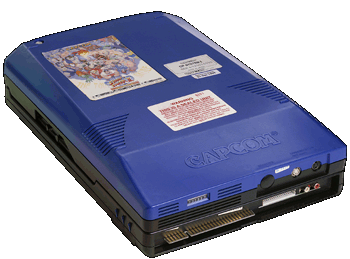
\includegraphics[height=40mm]{Reference/cps2.png}
\caption{A CPS2 B-board}
\label{fig:xbox360}
\end{center}
\end{figure}

Additionally, since the manner of the encryption was also secret, even when a method was developed to read the encryption keys off of the games B-board, they would be useless without knowing the exact encryption system used. It was determined however, much later on, that the encryption system used across all CPS-2 games was the same. This was likely due to cost concerns. Since the encryption system used custom developed hardware, it would have been cost preventative to develop and manufacture multiple different versions. Since all secret information used in this encryption system is contained somewhere on the distributed B-board, the system was vulnerable to several techniques which were used to eventually break the systems encryption.


\subsection{The Breaking of the CPS-2 system}
The first question about breaking the CPS-2 system one could ask is, why bother? Arcade systems are becomingly increasingly obsolete, and manufacturing bootleg CPS-2 systems is no longer economically viable. There are 2 main drivers behind the cracking of the CPS-2 system.

\begin{enumerate}
\item
As has already described, CPS-2 B-boards commit suicide when their batteries run out. Until the CPS-2 system was broken, the only way to repair these boards was to ship them to Capcom for servicing. Owners of CPS-2 systems clearly desired means to repair dead boards on their own

\item
A passionate community of Arcade System enthusiasts has developed an arcade emulator, the Multiple Arcade Machine Emulator (MAME). This software allows anyone with a PC to emulate historical Arcade Systems using PC hardware and software. The developers of this tool want as accurate as possible emulation of past Arcade Systems.

\end{enumerate}


The analysis and breaking of the CPS-2 encryption system is attributable to multiple parties. Information about the details of the process are sketchy at best and had to be pieced together from multiple sources including internet websites, forums and source code.  The main driver behind the process however was the CPS-2 shock team, initiated in the late 1990�s. This team was put together for the purpose of developing methods of understanding and manipulating the CPS-2 system. Their first product was an interface between the CPS-2 hardware and PC equipment. With this accomplished they were able to obtain memory dumps of working systems. Since some games were distributed on both the CPS-2 and CPS-1 system, this allowed for analysis of the CPS-2 decryption to commence. Eventually 2 intrepid hackers Nicola Salmoria, the main developer behind the MAME project, and Andreas Na�ve a Spanish programmer, were able to cryptoanalyze the CPS-2 encryption system and published their findings. The twists and turns this effort took are illustrative of other encryption breaking efforts, and we can discuss some of the details about how it came about.

\subsection{Cracking the CPS-2 System. }

Once the CPS-2 shock team had interfaced the CPS-2 boards to a PC, some details about the mechanism of encryption were released. Of the 16 MB in the CPS-2 address range, 4 MB are allocated to ROM game code and data. Approximately 1 MB of this is in an encrypted section.  The decryption machinery takes as input an address and the value of memory at that address. This means two things, first the decryption machinery must be extremely fast, since it is built in to the memory addressing of the system board. In fact the processor used is a modified Motorola 68000, which contained special instruction relating to the ROM encryption.  Because the CPS-2 used a 16-bit processor, the total number of combinations of plaintext were $2^{16}$ memory addresses $* 2^{16} $ 16-bit words. That is by running the encryption machinery using the total input space of $2^{32}$ values, and storing the $2^{33}$ bytes or 8GB of output data, tables could be produced which could decrypt running CPS-2 games in real time.  These tables were certainly unwieldy, especially considering that the actual game data from some of the CPS-2 games were thousands to millions times smaller then 8GB. This did, however, allow meaningful analysis of the tables to begin.

On January 15, 2006, Nicola Salmoria \cite{nicola} made the first breakthrough in understanding the CPS-2 system when he noted that,

\begin{verbatim}
sfzj\_049e38[x] $\oplus$ 0xFFFF == sfzj\_05ee0c[x $\oplus$ 0FFFF]
\end{verbatim}

In other words the CPS-2 encryption obeyed a complementation property which effectively chopped the decryption tables in half. This analsis began a year long investigation into the CPS-2 encryption system. The next step was to generate tables by flipping bits and examining the output, effectively performing differential cryptanalysis. This lead to the information that
\begin{quote}
Flipping bit 9 in the encrypted value causes bit 0 in the decrypted value to flip exactly 0x5080 times out of 0x10000, for every game, at every address.

This property is quite interesting. It is the most obvious "signature" of the algorithm. Does it help? Well, it tells us that if the algorithm contains bit permutations that depend on the key, those permutations cannot affect bits 3 and 9 in the encrypted value, nor bits 0 and 14 of the decrypted data.
\end{quote}

Nicola and Andreas Naive were able to hypothesize that the underlying algorithm used in CPS-2 was an even round Feistal network. This information coupled with above information about unaffected bits in the output of the network, demonstrating poor diffusion, allowed them to continue the differential cryptanalysis attack on the algorithm. \footnote{Andreas, who performed the bulk of the differential analysis is Spanish. The Google translation of his Spanish blog is surprisingly good, and allowed many of the details to be identified.}

Because Nicola and Andreas were reconstructing the Feistal network from generated tables, it is likely that the permutations, s-boxes and key schedule does not exactly match the actual network as programmed, but they do perform functionally identically. This allows the details of the CPS-2 encryption system to be practically realized.

The CPS-2 encryption system is a 4-round Feistal network with a 64-bit key. The key schedule expands the key out to operate like a 96-bit key. The system operates twice, once on the 16-bit address, then again on the 16-bit value.

\begin{quote}
1. Take the 16-bit address and a 96-bit key and run them through the first Feistel network, to produce a 16-bit subkey.

2 Take the 16-bit ciphertext, 16-bit subkey, and another 96-bit key and run them through the second Feistel network, to produce the 16-bit plaintext
\end{quote}

Once the algorithm was reconstructed, Nicola was able to devise a meet-in-the-middle attack on the algorthim to determine the 64-bit game key for games of which a full dump was available. This approach relied again on the poor diffusion offered by the CPS-2 Feistal network. By February of 2007 all of the details of CPS-2 encryption system had been made public.


\subsection{Lessons from CPS-2}
Capcom clearly learned their lesson. After rampant piracy of their CPS-1 system, the CPS-2 was completely effective in its goals of stopping piracy. However the system was vulnerable to a number of techniques and was ultimately cracked years after its effective life was over. The CPS-2 also represents an excellent balance of hardware versus software encryption. Some encryption systems rely upon that fact that an attacker will have limited understanding of custom hardware. These systems are rarely successful because given enough time an effort a dedicated hacker will build up enough information about a hardware system to effectively compromise it. Software systems are clearly desired but often times operate to slowly to be useful. In the CPS-2, since the encryption hardware was running off of the address bus, it needed to be extremely efficient. This limited the number of rounds that the encryption could employ, leaving the algorithm open to differential cryptanalysis. In fact the hardware was just efficient enough to perform its job of preventing bootlegging at the time of its production. Capcom engineers could have spent more time and money securing the system against attacks in the indefinite future. This would ultimately have resulted in a system which would have been more expensive and later to market. This balance of efficiency versus cost will be repeated for the next two systems we�ll be discussing.

Another lesson that will come into play with the later systems discussed is that there a wealth of brilliant engineers who will attack an encryption system, especially of popular systems. In the face of such competition perhaps the best outcome will be if the system protection is able just strong enough to slow down attacks until another system can replace it.

\section{The Microsoft Xbox}
The Microsoft Xbox was introduced in 2001 as a direct competitor to the Sony PlayStation 2, which was already an extremely popular system following an even more popular system the PlayStation 1. Because Microsoft lacked experience in the home console market, the decided to leverage their overwhelming experience in the IBM PC architecture coupled with their existing DirectX graphics libraries on that platform to speed the development of the Xbox. The resulting Xbox was, for all intents and purposes, a low cost personal computer. This presented a dilemma to Microsoft. They needed to use already available computer components to develop their system in time to compete with the PlayStation 2, but this left little room to secure their system against unauthorized hacking that was going to be inevitable when the system was introduced to the public. Microsoft ended up going with a system that was similar in nature to the CPS-2, and likely would have been effective if not for the interest of an relentless hacking community.

\subsection{The Xbox Hardware}
The Xbox utilized a stock Pentium 3 processor with a slightly modified graphics card. Many of the parts used in the Xbox were commodity components, one of the key exceptions being the NVidia Southbridge  chip used for low speed IO. This was connected to the processor over a Hypertransport bus. Hypertransport is a standard bus interface frequently used to connect computer components.

\begin{figure}[h]
\begin{center}
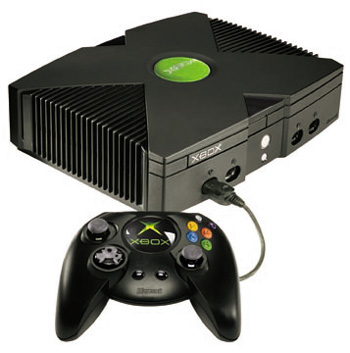
\includegraphics[height=40mm]{Reference/xbox.jpg}
\caption{A Microsoft Xbox}
\label{fig:xbox}
\end{center}
\end{figure}

The Xbox was also the first game console to ship with a mass storage device. Each Xbox included a 8GB hard drive on which was stored save games and downloaded content.

\begin{center}
\begin{tabular}{|l|l|}
\hline
\multicolumn{2}{|c|}{Xbox Hardware Details} \\
\hline
Main CPU & 733 MHz Intel Pentium III-based Mobile Celeron \\
GPU &233 MHz nVidia NV2A \\
Peak Triangle Performance &  970,833 triangles per frame at 30fps \\
Storage & 8 or 10 GB, 3.5 in, 5,400 RPM hard disk. Formatted to 8 GB \\
Audio Process & NVIDIA "MCPX" \\
Resolution  & 480i, 576i, 480p, 720p and 1080i \\
\hline
\end{tabular}
\end{center}

\subsection{Xbox Live}
The Microsoft Xbox was also revolutionary in the extent to which it was connected to the Internet. Microsoft launched an online service, called Xbox live which connected Xbox owners around the world and allowed them to play against each other in online games. There are a number of cryptographic protocols in use to secure the Xbox live network, which are not going to be discussed here. What is interesting about Xbox Live from a hardware security perspective is that Xbox Live allowed Microsoft to transmit updates to the Xbox�s onboard software packages remotely. Microsoft made extensive use of this, and in fact access to Xbox Live is predicated on users allowing Microsoft to update their systems Software to the latest versions. All pervious gaming systems were launched with onboard software which was practically unchangeable. Microsoft, understanding that vulnerabilities would be discovered after the system�s launched, wanted to allow themselves a mechanism to patch security vulnerabilities without modifying the hardware or the manufacturing process.

\subsection{The Xbox Encryption system 1.0}
Microsoft engineers clearly took protection seriously when they designed the Xbox encryption system. Their system ultimately was unsuccessful not because of a fundamental disregard for security, rather on their schedule prohibited them from designing and integrating enough custom security hardware to prevent hackers from gaining access to crucial security information.

There were multiple reasons for cracking the Xbox security system. Since the Xbox was designed as a low-cost PC, there were a wide number of open-source compilers and tools capable of producing software designed to run on the Xbox. Also, since Microsoft was selling the Xbox at a loss, so as to compete with the PlayStation 2, the Xbox was viewed as a potential low cost general purpose computing machine. Microsoft, however, generates revenue in its gaming division by selling games; each Xbox converted to be used as a computer represents lost revenue to Microsoft. Microsoft employed a system to prevent such conversions from happening. This system also prevented users from playing copies of games produced by consumer DVD burners.

The design of this system was much more involved than in the systems that the Xbox was competing with, the PlayStation and the PlayStation 2. Because these systems used more custom hardware, and they didn�t ship with a hard drive, the main threat was of pirates producing copied games. Sony protected against this with a simple switch from the CD (or DVD drive in the case of the PlayStation 2) to the CPU. This line identified the disc as genuine or not by reading information on the disc, in a place not accessible by normal consumer CD/DVDS burners. This mechanism was cracked by soldering �mod-chip� devices over this line. These chips were widely produced and available.

The Xbox protection is a layered defense. Since the Xbox loads and runs code produced by third parties on DVD-ROM discs, the first layer is authentication on the DVD-ROMS. The DVD-ROM security is designed to prevent 2 kinds of unauthorized access. First, Microsoft wants to prevent users from compiling their own code, burning it onto a DVD and loading it into the Xbox. To this end each DVD-ROM contains a security section which is signed by a 2048-bit RSA key. This forces users to hand over their DVD to be signed by Microsoft using their private key before they can distribute and load Xbox code. Although a 2048-bit key is extremely large there was a distributed computing project which was started with the purpose of factoring the Xbox public key to obtain Microsoft�s private key. This project continued for several years but was ultimately abandoned.

Second, Microsoft wants to prevent users from copying already signed discs, thereby allowing them to play pirated copies of games. This protection is built into the hardware of the DVD-ROM. The DVD is able to identify the kind of media inserted, this is encoded on the disc itself. Users are unable to obtain discs encoded with the Xbox code, thereby preventing them from loading copied discs.

Since the Xbox kernel will only load games signed with Microsoft�s private RSA key, the next avenue of attack is the kernel itself. If users can bypass the normal loading mechanism, inserting their own firmware code, they would be able to run arbitrary code on the Xbox. Additionally, since the Pentium 3 x86 platform the Xbox was designed with is an extremely well-documented and widely used platform, there is an extensive amount of tools for debugging and engineering x86 platforms.  This is in contrast to the CPS-2 system, where it took months to years just to engineer equipment that could connect CPS-2 hardware with a PC.
The Xbox 1.0 boot process is descibed in detail in \cite{huang-xbox}.

\begin{enumerate}
\item
Upon start up a secret ROM located in the Xbox southbridge is activated. This ROM contains enough code to run a tiny virtual machine. This machine can run simple instructions called XCodes  (or Jam Codes) which can read and write to memory, but is limited in the address space they can access

\item
The virtual machine loads XCodes from a programmable flash chip on the motherboard. This initializes the Xbox. Once initialized the Xbox kernel is decrypted and loaded into memory. The Xbox 1.0 kernel was encrypted using the RC4 stream cipher with a 128 bit key. The cipher key is located in the secret ROM chip on the southbridge.

\item
Once the kernel was RC4 decrypted, the secret chip was deactivated, preventing hackers from accessing it. This was essential to ensuring the security of the RC4 key.

\item
Once decrypted the kernel continued the boot process, eventually verifying the RSA key on an inserted game disc and running the game.

\end{enumerate}


The Xbox security relied in large part upon the secret ROM chip. Information was placed onto the NVidia south bridge for two reasons. If the Xbox designers had used a standard flash chip it could have been easily replaced by Xbox hackers. By placing it on a custom chip, Microsoft ensured that hackers could not gain access to aftermarket chips, thereby circumventing the security. Second, since the Xbox south bridge chip was one of the few custom chips build explicitly for the Xbox, this allowed them to place custom storage onto the chip.

The crucial mistake made in this implementation was the use of RC4 in the decryption of the kernel. If the 128-bit key can be kept secret, then no-one would be able to replace the installed firmware. However because RC4 is a symmetric cipher, the key had to be located somewhere on the Xbox system. Microsoft designers assumed it would be impossible to extract the key.

Microsoft�s assumption was proven incorrect by Andrew Huang, who successfully tapped the hyper-transport bus between the CPU and the south bridge chip. This was previously believed to be impossible. He then wrote a program which logged all communication between the CPU and the southbridge chip during bootup. Since the key had to be transmitted in that time, he was able to locate the RC4 key used for kernel decryption. The publishing of this RC4 key allowed anyone to overwrite the installed Xbox kernel with custom code (provided that someone had access to a flash programmer). This ended the life of the Xbox 1.0 security system. Microsoft immediately responded by trashing the existing southbridge chips and replacing them with what has become known as Xbox security 1.1

\subsection{Microsoft Xbox Security 1.1}
Once the RC4 key was made public the Xbox 1.0 security was eliminated. The Xbox 1.1 system used an almost identical hardware system as the original Xbox 1.0. The major difference was the mechanism used to verify the Xbox kernel. Since Microsoft now knew that all communications on the Xbox were insecure, they replaced the RC4 cipher with a hash. The secret southbridge chip performed a hash against the Xbox kernel. It then compared this hash to a value stored on the southbridge. As mentioned earlier, the south bridge was effectively irreplaceable by hackers due to its custom components. This guaranteed the security of the hashed value.

Unfortunately for Microsoft, they made even more crucial mistake in their hashing algorithm then they did with the RC4 implementation. Because space on the south bridge chip was extremely limited, they would unable to fit a full-featured hashing implementation like MD5 or SHA-1 on the chip. Instead they went with the lightweight Tiny Encryption Algorithm (TEA). What the designers failed to realize was that TEA contained a crucial disclosed vulnerability, and as a result should never be used as a hash.

When TEA is used as a hash, two adjacent 32 bit values can be modified in the high order bit without affecting the ultimate hash value. This provided just enough breathing room for hackers to break the security. This was discovered by Andy Green, where he was able to modify the appropriate bits of a jump instruction to jump into RAM outside of the Xbox kernel. This gave him complete control over the box.

\begin{quote}
But why did they make this mistake? Obviously the designers knew nothing about crypto - again! - and just added code without understanding it and without even reading the most basic books on the topic. A possible explanation why they chose TEA would be that they might have searched the internet for a "tiny" encryption algorithm - and got TEA. \cite{mistakes-xbox}
\end{quote}

\subsection{Other Xbox Vulnerabilities}
There are a number of other Xbox vulnerabilities which bypass the Xbox encryption rather then attack it head on. This includes some hardware bugs that allow users to prematurely turn off the secret south bridge chip, or to access the secret southbridge chip before it is turned off.

There is one other interesting class of vulnerabilities that play a role in the Xbox�s successor, save game exploits. Most modern video games save some sort of data to persistent storage. Bugs in the loading of these save game states can lead to buffer overflows which allow for arbitrary code execution. A  number of Xbox games suffered from these vulnerabilities including MechWarrior and GoldenEye. They are very desirable from a hacker standpoint because they require no hardware modification, whereas changing the Xbox firmware requires removing and replacing the flash chips located on the motherboard.  Since original Xbox games all ran in kernel mode, once a user had found a save-game exploit they were able to effectively control the Xbox.

A number of these vulnerabilities were patched through Xbox Live. Microsoft played a cat and mouse game with hackers for a number of years, patching one vulnerability after another. The end of the commercial life of the Xbox moved the playing field to the Xbox 360.

\subsection{Lessons from the Xbox security system}

There are a number of lessons to be learned from the original Xbox security system. Microsoft was unable to strike the right balance between custom components and cost in their design. They underestimated the resources of the hacking community.  By relying on the south bridge chip for their security system, Microsoft was unable to ultimately secure the Xbox. Also they couldn�t rely upon third party software developers for the security of their system. Running games in kernel mode would eventually lead to exploits which could bypass the security.  And in fact there were even some exploits located in the font-rendering engine of the Xbox dashboard application that was written by Microsoft which could be taken advantage of by hackers. So an even stricter conclusion is that running code running in privileged mode is vulnerable. Microsoft would attempt to address these issues and more in the development of the Xbox 360.

\section{The Xbox 360}
The Xbox 360 was introduced in the 2005 as the successor. It ended the production of the original Xbox, which enjoyed a surprisingly short life-cycle when compared to other game consoles. The premature termination of the original Xbox was likely due to the complete ineffectiveness of the original Xbox security systems.  The Xbox 360 contained completely revamped security system, which contained some hints of the original Xbox system, but is much more secure.

\begin{figure}[h]
\begin{center}
\includegraphics[height=40mm]{Reference/xbox360.jpg}
\caption{The Xbox 360}
\label{fig:xbox360}
\end{center}
\end{figure}

\begin{center}
\begin{tabular}{|l|l|}
\hline
\multicolumn{2}{|c|}{Xbox 360 Hardware Details} \\
\hline
Main CPU & 	3.2 GHz PPC Tri-Core Xenon \\
GPU & 500 MHz ATI Xenos \\
Peak Triangle Performance &  500+ million triangles/sec. \\
Storage & Available 20GB Hard Drive\\
Audio Process & Handled on Main CPU\\
Resolution  & 720p \\
\hline
\end{tabular}
\end{center}

\subsection{The Xbox 360 Security System}
The Xbox 360 security system has been under study for that past several years without a severe vulnerability being found. There have, however, been a number of exploits located that have compromised the ultimate security of the box. The primary place for information and discussion regarding the Xbox 360 security system is the Xbox Hacket forums.

The Xbox 360 secures the DVD-ROM in the same manner as the original Xbox, with a 2048 RSA key. The Xbox 360 goes even farther in this protection by requiring all executables to be signed with the RSA key before being executed. The DVD-ROM drive located in each Xbox- 360 also contains a unique key. This is to prevent modification of the Xbox 360 with 3rd party DVD-ROM drives with modified firmware that bypasses the copy protection. Despite this protection it is possible to replace the Xbox 360 DVD-ROM drive since the security implemented by the 3rd party DVD manufacturer is not complete.  The details of this exploit have not been released since it can only be used to play pirated and copied games.

Initially hackers attempted to attack the Xbox 360 in the same manner as the original Xbox, by attacking the boot sequence. The Xbox 360 boot process is largely the same as the original Xbox, with a few crucial difference. Details are described in \cite{xbox360-boot}

\begin{enumerate}
\item
Upon boot-up, the ROM (1BL) code located \textbf{on the CPU itself} decrypts the second bootloader (2BL) using RC4. The 1BL also verifies the signature of the 2BL, details on the nature of the 2BL signature are not easily located.

\item
The 2BL (and subsequent bootloaders) decrypt the Xbox 360 Key Vault (KV) using a \textbf{per CPU-key} and  128-bit HMAC-SHA1. The key vault contains information like the DVD-Rom hardware key, console certificates and per-box keys.

\item
The 2BL loads the Xbox 360 Hypervisor into memory. The Hypervisor is signed and tagged with a fuse count number in the same manner as the key vault. The Hypervisor will fail to load if the fuse count number stored with the Hypervisor does not match the hardware configuration

\item
The Hypervisor transitions the CPU to user mode. All future requests for kernel-mode access require servicing by the Hypervisor.
\end{enumerate}

There are several pillars to this security system. First, the secret ROM on the south bridge chip has been replaced with code stored on the CPU. This is in direct response to the tap on the Hypertransport in the original Xbox. With no bus to tap this, information cannot be easily obtained. Second, a per-cpu key is used to decrypt key parts of the system including the key-vault and the Hypervisor, this prevents someone from finding and releasing the encryption keys. Both of the components are protected with a 128-bit HMAC-SHA1. Thirdly the hash on the 1BL has apparently been made secure, and no long relies upon TEA.

\subsection{The Xbox 360 E-Fuse}
One of the most important changes to the Xbox 360 security system is located on the CPU. The Xbox 360�s PowerPC processor contains a feature know as E-fuse. These are programmable fuses readable using special CPU instructions. There are several hundred E-fuses, used to provide two layers of security.

First, the E-Fuses contain a unique, per-CPU key readable only while the CPU is in kernel mode. In practice this means the CPU key is protected by the Hypervisor which limits box access to kernel mode features. The CPU key is used to encrypt and sign several key data structures. This prevents a lone hacker from determining the key for all Xbox 360 users. The determination of the key must happen on a per-CPU box (if it can happen at all).

Second, Microsoft installed a resistor on the Xbox 360 motherboard which enables the CPU to modify, or blow, E-fuses programmatically, this resistor is show in Figure~\ref{fig:xbox360resistor}. Since the Xbox 360 is a networked device, and connected to the Microsoft Xbox Live network, there are frequent kernel updates, especially when the security of the kernel has been compromised. Each kernel is verified against the E-fuse count before allowed to load. By blowing E-fuses when performing kernel updates, Microsoft ensures that users cannot downgrade the Xbox kernel software to a more vulnerable version after it has been upgraded. For example, when an Xbox 360 console is upgraded kernel version 4548 to 4552, an E-fuse is blown on the device that prevents versions previous to 4552 loading. This is enforced by a secure check performed at boot-up. Specifically an e-fuse sequence number is stored in the kernel data section of flash memory at byte 0x021F. This section of memory, from 0x00 to 0x220 are hashed using the CPU key and verified by the 2BL, the hash is stored at memory location 0x220. Any attempts to modify the sequence number will break the hash. With the CPU key, the hash can be recreated by anyone. Any attempt to load kernels where the sequence number is less then the number of available E-fuses on the system result in a non-functioning (bricked) box.

\begin{figure}[h]
\begin{center}
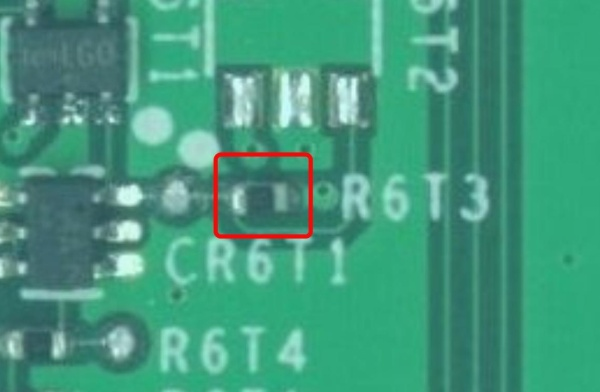
\includegraphics[height=40mm]{Reference/r6t32.jpg}
\caption{The R6T3 resistor allows Microsoft to programmatically blow E-fuses}
\label{fig:xbox360resistor}
\end{center}
\end{figure}


\subsection{Attacks on the Xbox 360}
As has been described the Xbox 360� security system was much more developed then the original Xbox. The addition of the CPU E-fuses made any progress substantially more difficult. Also, the presence of the Xbox Hypervisor made any attempt execute code and obtain the E-fuse information theoretically impossible; nevertheless, attacks do exist on the Xbox system.

The first vulnerability discovered for the Xbox was what is known as the King Kong exploit. King Kong was a launch title based upon the movie of the same name. While we have already discussed the fact that all Xbox DVD�s are signed with a 2048-bit RSA key, and furthermore all executable code is also signed with the same key there are attacks on the signing system. In the interest of performance the Xbox DVD signs only DVD header information. This allows some modification to DVD data without affecting the signature. This allows Xbox games to more effectively load game content, meaning 3D model, artwork, and sound files, without incurring the overhead of a RSA signature verification step. Only executable files are fully signed, preventing modification to their data.

King Kong made use of a number of Vertex Shader programs. These are small programs designed to run solely on the graphics card of the Xbox, mostly for the purpose of adding graphical effects. Probably to ease development, the King Kong programmers decided to store the King Kong shader files in plain text on the King Kong DVD, then dynamically compiling them during runtime. Because these files blurred the line between game content and game executable, they were not signed as part of the game production process. This allows attackers to make small modifications to the shader files, inserting their own instructions. The Xbox�s graphics card is also extremely powerful, and it can execute instructions which modify areas of memory. The combination of all these factors allowed attackers to run arbitrary code on the Xbox 360.

At this point the first layer of defense has been broken. By using the King Kong exploit attackers can run arbitrary code on the Xbox. This kind of attack is very similar to the save game attacks discussed earlier, and was the exact reason the Xbox Hypervisor was developed. Even though attackers could run arbitrary code on the Xbox, they were prevented from executing privileged instructions on the 360 due to the Hypervisor protections. In particular attackers cannot gain access to the E-fuse information because this requires privileged access.

Unfortunately for Microsoft, the Hypervisor itself contained vulnerability. The second exploit discovered was in the Xbox Hypervisor version 4548 in February 2007 \cite{security-focus}. It was discovered that a privileged escalation bug existed in the Hypervisor.

\begin{quote}
The problem is that the "cmplwi" instruction compares only the lower 32
bits of the given syscall number; the upper 32 bits are ignored. The
"rldicr" instruction, however, operates on the complete 64 bit register
value.
\end{quote}


The result of this is that by executing carefully crafted rldicr (Rotate Left Double Word Immediate then Clear Right) instructions hackers could bypass the Hypervisor and gain access to privileged execution set. This allowed them to gain access to the CPU E-fuse data, which would further allow them to alter the values of the Key Vault and 2BL to values of their choosing. With the E-fuse information they could then recreate the signatures for those sections of memory.

The Hypervisor vulnerability was not released until after Microsoft had already released a patch via Xbox live. The new version of the Hypervisor 4552 patched the Hypervisor exploit. Additionally, as was already mentioned, this update blew an E-fuse making it impossible to load previous/vulnerable versions of the Hypervisor. The result of this was that the vast majority of existing Xbox 360�s were running patched kernels. It is also worth noting that because all Xbox 360 games are signed with the same key, there can be no per-game key revocation. This prevents Microsoft from ever patching the KK exploit. The Sony PlayStation 3 and it associated Blu-Ray protection does include a key-revocation procedure in case hardware keys are ever compromised.

Hackers were in a quandary at this point. They KK exploit coupled with a vulnerable Hypervisor could bypass all of the Xbox security restrictions, but they would only work on older Xbox 360 which had not been patched. The next exploit was aimed at this problem, and allowed hackers to boot older kernels. In July of 2007 a hacker called arnezami hypothesized that the SHA1-HMAC used to verify that E-fuse kernel matching might be vulnerable to timing attack. Since the memory compare function in the 1BL performed a byte-wise compare, short-circuiting the comparison if a match was not found, if it was possible to measure the time it took to do the comparison, then the hash might be successfully bypassed.
A month later the attack was successfully implemented. The attack goes as follows

\begin{enumerate}
\item
Load a vulnerable kernel into the Xbox 360 flash. The 16 byte SHA1 hash value used to verify the E-fuse count will be incorrect.

\item
Build custom hardware capable of microsecond timing resolution. Also a flash programmer is required to cycle each byte through all possible values.

\begin{figure}[h]
\begin{center}
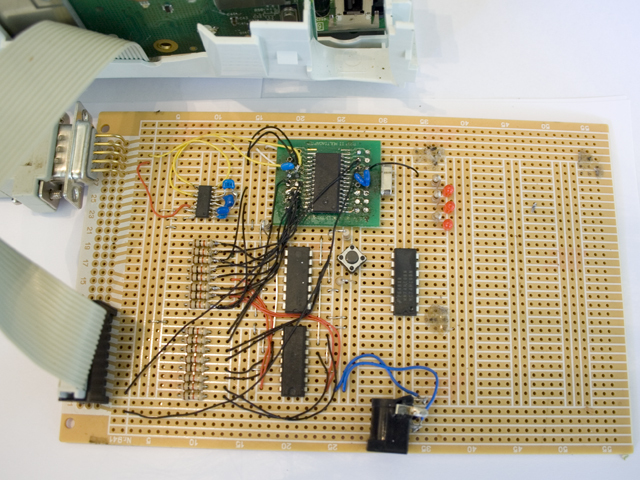
\includegraphics[height=50mm]{Reference/timing.jpg}
\caption{This hardware is required to perform the timing attack against an Xbox 360}
\label{fig:timing}
\end{center}
\end{figure}

\item
Run through all values on the first byte of the hash. Locate the value which caused the Xbox 360 the longest time to fail. Set the first value of the hash to that found value and move on to the next byte. This allows a 16-byte hash to be determined in 256 * 16 = 4096. There is a hardware issue here in that the Xbox 360 flash has a limited write lifetime, however this operation needs only to be completed once. Once the hash value is correct the 2BL will load a vulnerable kernel.

\end{enumerate}

The vulnerable code lives in the 2BL, which is verified against a hash stored in the CPU. It is unlikely to ever change, since this would require reprogramming the Xbox 360 CPU, a potentially very expensive procedure. Once the vulnerable kernel is loaded, the King Kong exploit coupled with the Hypervisor exploit will lead to the E-fuse data at which point the flash can be completely reprogrammed.

\subsection{Lessons from the Xbox 360 Security System}
The lesson from the Xbox 360 is that the chain of trust in such complicated systems is brittle and difficult to secure. While every component used to secure the Xbox was cryptographically secure including the use of RSA authentication and cryptographic signing, RC4 with strong keys, SHA1 with 160-bit hash, the seams which tied these measures together were vulnerable to attack. TheSpecialist, one of the key hackers working on the Xbox 360 described the techniques as follows:

\begin{quote}
The idea of the Hypervisor and certainly the fuses is simply genius. Putting the bootrom in the CPU was also a real good idea. All communication is encrypted as it should be. Even now we can dump and decrypt all program code and nothing is really 'secret' anymore we still can't run unsigned code on the new kernels. I think that says a lot.
\end{quote}

The Xbox designers clearly approached security in a comprehensive way, but due to minor failures in the some security subsystems, the security of the whole system was violated. They did accomplish a great deal in that over 2 years since the Xbox 360 launch there is still no general purpose hack for the Xbox 360. The attacks described above all require custom built hardware in order to modify the internal memory of the Xbox 360. Certainly the timing attack is challenging to perform, and once an Xbox has been modified, it can never be connected to Xbox Live again, since the changes to the system could be easily detected by the Xbox Live servers. This situation was completely different for the original Xbox, which could essentially be modified by anyone. The Xbox 360 can still only be modified by reverse engineering experts, and under controlled conditions.



\section{Conclusion}
Can a secure system ever be produced? This likely a pipe dream, the fact of the matter is that the gaming systems in use today are designed by hundreds of people and rely upon thousands of components. A flaw in any single hardware component, or a line of code, will lead to an exploitable system. Preventing this from happening would be so cost intensive as to the render the developed system unaffordable, and as a result systems will likely continue to be exploited. So for the foreseeable future, hardware designers will likely have to achieve the perfect balance of performance, security and cost in order to develop and ship successful game consoles.

\pagebreak
\nocite {*}
\bibliography{Encryption}
\bibliographystyle{is-alpha}

\end{document}
